\documentclass{beamer}

%%%%%%%%%%%%%Solarized Theme%%%%%%%%%%%%%%%
\usecolortheme[dark,accent=cyan]{solarized}
\beamertemplatenavigationsymbolsempty
%%%%%Packages%%%%%
\usefonttheme{serif}
\usepackage[T1]{fontenc}
\usepackage[utf8]{inputenc}
\usepackage[english]{babel}
\usepackage{fontawesome}
\usepackage{minted}
\usepackage{soul}
\usepackage{ulem}
\usepackage{blkarray}
\usepackage{multirow}

\definecolor{DarkGray}{gray}{0.1}
\usemintedstyle{paraiso-dark}


\usepackage{graphicx}
\usepackage{hyperref}
\usepackage{colortbl, xcolor}
\usepackage{booktabs}
\usepackage{amsmath,amsthm, amssymb, latexsym}

\usepackage{tikz}
\usepackage{xcolor}
\usepackage{graphicx,multirow}
\definecolor{plain}{rgb}{93,93,93}
\usetikzlibrary{positioning,arrows}
\definecolor{applegreen}{rgb}{0.55, 0.71, 0.0}
\usetikzlibrary{decorations.pathreplacing, backgrounds, fit}
\usetikzlibrary{calc,matrix}

\tikzstyle{background}=[solarizedRed, rectangle, draw, inner sep=1mm, thick,
           rounded corners=2mm]

\tikzset{
  treenode/.style = {align=center, inner sep=0pt, text centered,
    font=\sffamily},
  arn_n/.style = {treenode, circle, white, font=\sffamily\bfseries, draw=black, inner sep=-6pt,
    fill=black, text width=1.5em},% arbre rouge noir, noeud noir
  arn_r/.style = {treenode, circle, red, 
    text width=1.5em, very thick, inner sep=4pt},% arbre rouge noir, noeud rouge
  arn_x/.style = {treenode, rectangle, draw=black,
    minimum width=0.5em, minimum height=0.5em}% arbre rouge noir, nil
}

\usepackage{standalone}
\usepackage{siunitx}

\begin{document}

\begin{frame}
    \begin{center}
        \Large{\textcolor{orange}{It's Payback Time: New Insights on Cooperation in the Repeated Prisoners' Dilemma}} \\
    
        \vspace{1cm}
        \normalsize{@NikoletaGlyn} \\
        \vspace{.5cm}
        
\includegraphics[width=0.14\textwidth]{static/dyno.png}

    \end{center}
\end{frame}

\begin{frame}
    \begin{center}
        \LARGE{\textbf{Why?}}
    \end{center}
\end{frame}

\begin{frame}
    \begin{center}
        \LARGE{``Slow to anger and fast to forgive: Cooperation in an uncertain world''} \\ \vspace{.5cm}
        \normalsize{Drew Fudenberg, David G. Rand, Anna Dreber}
    \end{center}
\end{frame}

\begin{frame}
    \centering
    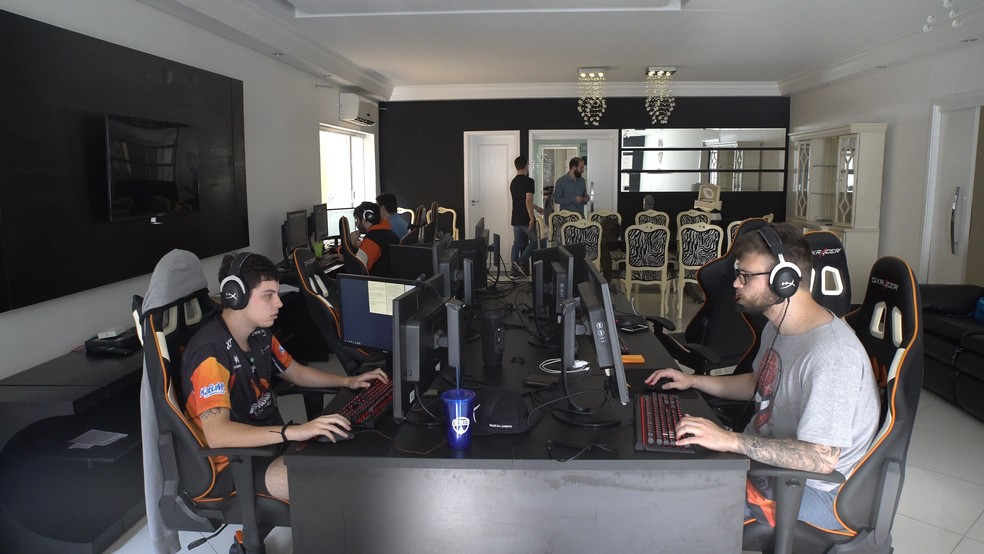
\includegraphics[width=.85\textwidth]{static/experiment}
\end{frame}

\begin{frame}
    \centering
    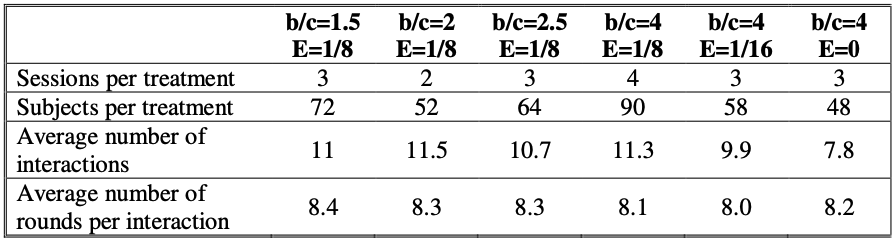
\includegraphics[width=.85\textwidth]{static/setup} \\
    \hspace{6cm} \textit{(original paper)} \vspace{2cm}

    \pause
    \hspace{6cm} \textbf{count: 1}
\end{frame}

\begin{frame}
    \centering
    \textbf{Finding A:} Although not an equilibrium strategy, TFT is empirically
    widely used both with perfect and imperfect monitoring (p.734 and Table 3 in
    FRD).
\end{frame}

\begin{frame}
    \centering
    Maximum Likelihood Estimation \\\vspace{.5cm}
    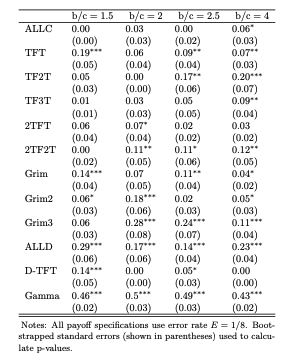
\includegraphics[width=.45\textwidth]{static/result A.png}
    \vspace{1cm}

    \pause
    \hspace{6cm} \textbf{count: 2}
\end{frame}

\begin{frame}
    \centering
    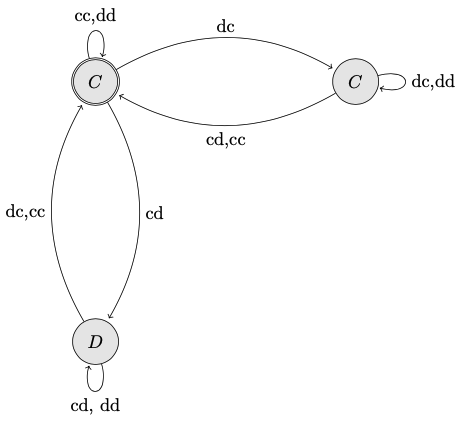
\includegraphics[width=.75\textwidth]{static/payback}
\end{frame}

\begin{frame}
    \centering
    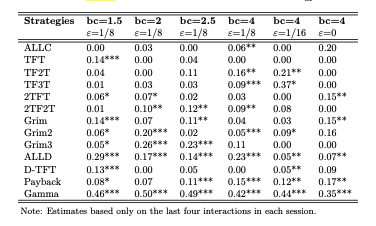
\includegraphics[width=.75\textwidth]{static/result A.1.png}
\end{frame}

\begin{frame}
    \begin{center}
    \LARGE{Nash Equilibrium}
    \end{center}
\end{frame}

\begin{frame}
    \centering
    \textbf{Finding B} The data do not show the strong support for risk
    dominance of TFT as the key determinant of the level of cooperation in
    games with noise that was seen in studies of games without noise (p.733 in
    FRD).
\end{frame}

\begin{frame}
    \begin{center}
    \LARGE{\textbf{Risk Dominance (?)}}
    \end{center}
\end{frame}

\begin{frame}
    \begin{center}
    \LARGE{``On the Determinants of Cooperation in Infinitely Repeated Games''} \\ \vspace{.5cm}
    \normalsize{Pedro Dal Bó and Guillaume R. Fréchette}
    \end{center}
\end{frame}

\begin{frame}
    \begin{center}
    ``A strategy is risk dominant if it is a best response to the other player
    randomizing 50 - 50 between the two strategies."
    \vspace{2cm}

    \pause
    \hspace{6cm} \textbf{count: 3}
    \end{center}
\end{frame}

\begin{frame}
    \centering
    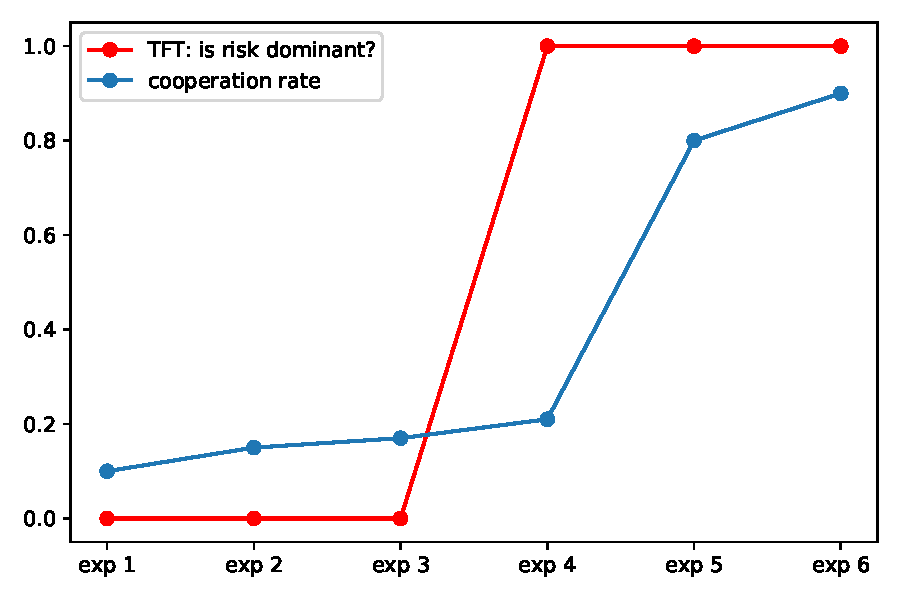
\includegraphics[width=.75\textwidth]{static/tft_rd.pdf}
\end{frame}

\begin{frame}
    \centering
    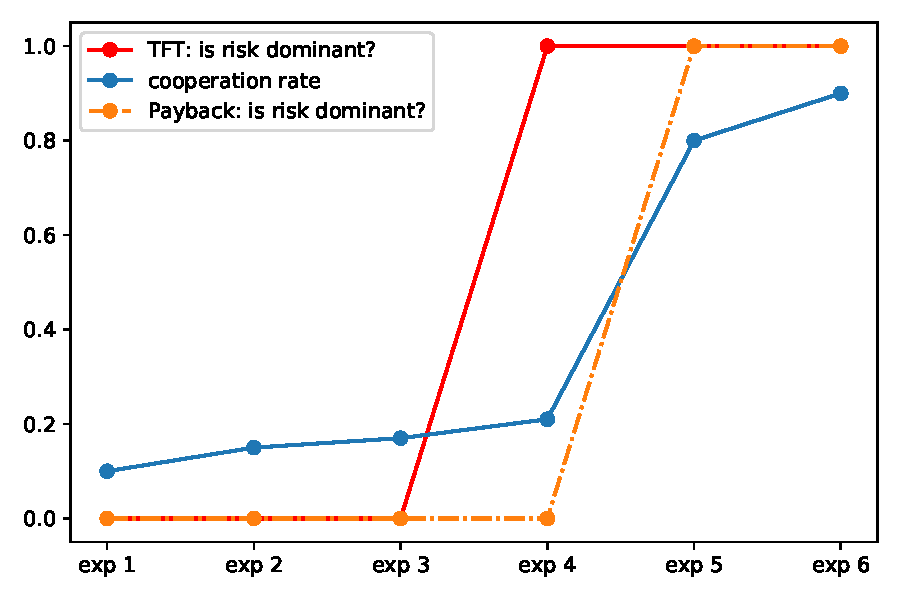
\includegraphics[width=.75\textwidth]{static/payback_rd.pdf}
\end{frame}

\begin{frame}
    \begin{center}
    \LARGE{\textbf{Conclusions}}
    \end{center}
\end{frame}
\end{document}